\documentclass{article}
\usepackage{fullpage}
\usepackage{graphicx}
\usepackage{../svn-multi}
\svnid{$Id: devguide.tex 10 2008-08-28 14:05:10Z jakebeal $}

\title{MIT Proto Developers Guide}
\author{Jacob Beal}
\date{Date: \today, SVN Version: \svnrev{}}

\newcommand\todo[1]{\immediate\write16{TODO: #1}}

\newcommand\fixme{{\bf NEEDS DEVELOPER ATTENTION}}

% proto code
\newcommand\code[1]{\begin{quote}\var{#1}\end{quote}}
\newcommand\function[2]
{\begin{quote}{\tt #1}: #2 \end{quote}}
\newcommand\type[1]{$#1$}
\newcommand\var[1]{{\tt #1}}

\begin{document}

\maketitle

This is a guide to developing for the MIT Proto project.  It outlines the
various components of the project, how they fit together, and how to
develop for them safely.

\tableofcontents

% standard LaTeX credits insert; should echo AUTHORS

\section{Credits for Proto}

The Proto language was created in partnership by Jonathan Bachrach and
Jacob Beal.  As they created the language, Jonathan created the first
implementation of MIT Proto, including the first compiler, kernel,
simulator, and embedded device implementations.  Since that time, Jake
and other contributors have built on the work begun by Jonathan.

MIT Proto also includes contributions from (alphabetically):
%
Aaron Adler, Geoffrey Bays, Anna Derbakova, Nelson Elhage, Takeshi
Fujiwara, Tony Grue, Joshua Horowitz, Tom Hsu, Kanak Kshetri, Prakash
Manghwani, Dustin Mitchell, Omar Mysore, Maciej Pacula, Hayes Raffle,
Dany Qumsiyeh, Omari Stephens, Mark Tobenkin, Ray Tomlinson, Kyle
Usbeck, Dan Vickery

The Protobo platform code in platforms/protobo/ also includes 
Topobo-related code from (alphabetically):
%
  Mike Fleder, Limor Fried, Josh Lifton, Laura Yip


\section{Overview}

Proto is a language designed for implementing distributed systems on
spatially-structured networks of static or mobile devices.  The
programmer describes a desired behavior for the continuous space
occupied by the network, which can be translated into a program by
which individual devices cooperate to produce an approximation of the
desired behavior.  Such programs can then be rendered into an
executable than can run equivalently on different hardware platforms.

\paragraph{Components}
MIT Proto is an implementation of Proto which supplies four main
components:
\begin{itemize}
\item A compiler which turns Proto code into executable code for
  individual devices
\item A library of Proto code implementing commonly used functions
\item An implementation of the ProtoKernel virtual machine, one means
  of executing programs on individual devices.
\item An event-based simulator, based on ProtoKernel, for debugging
  and visualization of Proto programs executing on a network
\end{itemize}

MIT Proto is typically invoked through one of two executables,
{\tt p2b} and {\tt proto}.  The name {\tt p2b} stands for ``Proto
to bytecode'' and is a standalone invocation of the compiler.  The
{\tt proto} executable, on the other hand, first compiles and then
executes in the simulator.

\begin{figure}
\centering
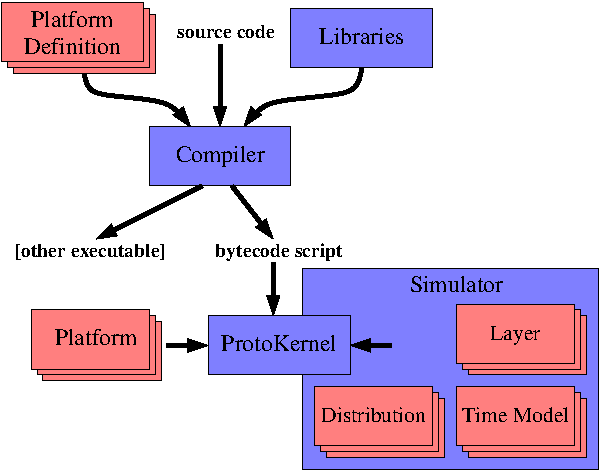
\includegraphics{figures/components.pdf}
\caption{Relationship of MIT Proto components (blue) and extensions (red)}
\label{f:components}
\end{figure}

% In simulator:
%   command line --> set of plugins, code, simulator platform file
%      code --> compiler --> bytecode
%      create VMs w. distribution, time model
%      event-based simulation: device evolution, layer evolution

% In real devices:
%   commandline + platform file --> p2b --> bytecode
%     devices compiled w. platform kernel
%     inject bytecode to one device, spreads virally


\paragraph{Extensions}
MIT Proto has interfaces allowing this system to be extended in three
ways:
\begin{itemize}
\item The compiler can emit code customized to different platforms
\item ProtoKernel can incorporate a set of platform-specific opcodes 
\item The simulator supports plug-in:
  \begin{itemize}
    \item Distributions for laying out the devices of a network (e.g.
      random, grid, torus).
    \item Models for the evolution of time on individual devices (e.g. 
      synchronous, drifting clocks)
    \item Physics ``layers'' for simulating the interaction of sensors
      and actuators with aspects of a dynamic external enviroment
      (e.g. wireless communication, chemical diffusion, Newtonian
      kinetics, LEDs and beeps)
  \end{itemize}
\end{itemize}

MIT Proto's is copylefted such that any modification of its components
is copylefted as well, but extensions need not be.

\section{Installed File Locations}

MIT Proto uses autotools to build and install on a machine.  By
default, the installation directory prefix is {\tt /usr/local/} (or
the OS-appropriate equivalent).  From this base, the following default
locations are used (reconfigurable via {\tt ./configure} when the project
is being built):

\begin{itemize}
\item Executables are placed in {\tt PREFIX/bin/}
\item The library files in the build directories {\tt lib/} and {\tt
    /lib/core/} are both placed into \\{\tt PREFIX/share/proto/lib}.
  This directory is part of the default search path for executions of
  the compiler.
\item Platform definition files for platform PLATFORM are expected 
  to be found in \\{\tt PREFIX/share/proto/platforms/PLATFORM}
\item The header files needed for building extensions for MIT Proto
  should be installed in \\{\tt PREFIX/include/proto/}, but currently
  are not. \fixme
\item Under the future plug-in system, the simulator should search for
  plug-ins in \\{\tt PREFIX/share/proto/platforms/sim/}
\end{itemize}

\section{Compiler}

This document describes only the compiler's interactions with other
pieces of the installation and its major known bugs.  The internal
structure of the compiler will not be documented in detail at this
time, because it is both highly complex and obsolete.

\paragraph{Compiling for a Platform}
The compiler loads platform-specific operations during its
initialization.  When given a \var{--platform {\it PLATFORM}}
argument, it reads the platform definition file {\tt platform\_ops.h}
from the platform directory for {\it PLATFORM} (see above).
This file is expected to contain C comments and a single enum of
the form: 
\code{
typedef enum \{\\
  {\it opcode-name} = CORE\_CMD\_OPS,\\
  {\it opcode-name},\\
  ...\\
  MAX\_CMD\_OPS\\
\} PLATFORM\_OPCODES;}
This file gives the compiler names and numbers for the opcodes to be
defined.

The compiler then reads the platform definition file {\tt
  platform\_ops.proto} from the same directory.  This is a Proto file
and is expected to contain a set of \var{defop} expressions of the
form: \code{(defop {\it opcode-name} {\it function-name} {\it type}
  ...)}  where {\it opcode-name} should match some entry in the {\tt
  platform\_ops.h} file (though they can be in a different order), and
{\it function-name} is the Proto function that will invoke the opcode.
The first {\it type} expression specifies the return type, and any
others that follow specify argument types for the operator.  The {\it
  type} expressions are currently allowed only to be one of
\var{scalar}, \var{boolean}, and \var{(vector 3)}.

\paragraph{Compilation and Files}

Compilation always starts with a Proto expression on the command line.
Except for the smallest of programs, this expression is not
self-contained.  Whenever the compiler encounters a function {\it
  name} that it does not know, it searches for a file called \var{{\it
    name}.proto} in the directories listed in its path.  By default,
the path consists of the current directory and the installed library
location.  These two command line arguments: \code{--path {\it PATH}}
\code{--basepath {\it PATH}} add to the default path and override the
default path, respectively.

\paragraph{Known Bugs}
Important known bugs in the current compiler are:
\begin{itemize}
\item Variables in a \var{letfed} that are not used within the body
  of the \var{letfed} are not updated correctly.
\item Variables in \var{let} statements that are used only within a
  conditional further on in the code are inlined inside that
  conditional, which makes side effects of the computation in the
  \var{let} happen only in the domain of that branch of the
  conditional.
\end{itemize}

\paragraph{Neocompiler}

A complete rebuild of the compiler is in progress, but not currently
checked into the repository. When complete, it will implement an
enhanced version of Proto, fix a number of known compiler bugs, change
how platform-specific opcodes are handled, and allow compilation for
execution on systems other than ProtoKernel.  \fixme{}

\section{Libraries}

MIT Proto includes two libraries: the functions in {\tt lib/} are
moderately complex programs that make useful buiding blocks, while the
functions in {\tt lib/core/} are language primitives implemented in
Proto.  They are mixed together in installation, but kept separate in
the build so that maintenance of the ``library'' collection is not
cluttered up by the large numbers of simple core functions like
\var{log10} and \var{logn}.  The core library exists because it helps
minimize the number of opcodes needed without hardwiring definitions
into the compiler.

\section{ProtoKernel}

\todo{Write ProtoKernel section}{\bf SECTION IN PROGRESS}

Built purely in C (no C++) for minimum size and maximum portability
across embedded platforms.

\section{Simulator}

\todo{Write Simulator section}{\bf SECTION IN PROGRESS}

Event-driven simulation

\begin{quote}
\begin{verbatim}
class EventConsumer {
public:
  virtual BOOL handle_key(KeyEvent* key) {return FALSE;} // return if consumed
  virtual BOOL handle_mouse(MouseEvent* mouse) {return FALSE;} // same return
  virtual void visualize() {} // draw, assuming a prepared OpenGL context
  // evolve moves state forward in time to 'limit' (an absolute)
  virtual BOOL evolve(SECONDS limit) {} // return whether state changed
};
\end{verbatim}
\end{quote}

\paragraph{Time}
real time vs. simulation time vs. device time

\paragraph{Visualization}

\subsection{Distributions}

\begin{quote}
\begin{verbatim}
class Distribution {
 public:
  int n; Rect *volume;
  METERS width, height, depth; // bounding box of volume occupied
  Distribution(int n, Rect *volume) { // subclasses often take an Args* too
    this->n=n; this->volume=volume;
    width = volume->r-volume->l; height = volume->t-volume->b; depth=0;
    if(volume->dimensions()==3) depth=((Rect3*)volume)->c-((Rect3*)volume)->f;
  }
  // puts location in *loc and returns whether a device should be made
  virtual BOOL next_location(METERS *loc) { return FALSE; } // loc is a 3-vec
};
\end{verbatim}
\end{quote}

\subsection{Time Models}

\begin{quote}
\begin{verbatim}
// a bit of state attached to a device to say how its time advances
class DeviceTimer {
 public:  // both of these report delay from the current compute time
  virtual void next_transmit(SECONDS* d_true, SECONDS* d_internal)=0;
  virtual void next_compute(SECONDS* d_true, SECONDS* d_internal)=0;
  virtual DeviceTimer* clone_device()=0; // split the timer for a clone dev
};
\end{verbatim}
\end{quote}

\begin{quote}
\begin{verbatim}
// factory class for producing DeviceTimers
class TimeModel {
 public:
  virtual DeviceTimer* next_timer(SECONDS* start_lag)=0;
  virtual SECONDS cycle_time()=0;
};
\end{verbatim}
\end{quote}

\subsection{Layers}

\begin{quote}
\begin{verbatim}
class Layer : public EventConsumer {
 public:
  int id;          // what number layer this is, for lookup during callbacks                    
  BOOL can_dump;   // -ND[layer] is expected to turn off dumping for a layer                    
  SpatialComputer* parent;
  Layer(SpatialComputer* p);
  virtual ~Layer() {} // make sure that destruction is passed to subclasses                     
  virtual BOOL handle_key(KeyEvent* key) {return FALSE;}
  virtual void visualize() {}
  virtual BOOL evolve(SECONDS dt) { return FALSE; }
  virtual void add_device(Device* d)=0;    // may add a DeviceLayer to Device                   
  virtual void device_moved(Device* d) {}  // adjust for device motion                          
  // removal, updates handled through DeviceLayer                                               
  virtual void dump_header(FILE* out) {} // field names in ""s for a data file                  
  virtual layer_type get_type() { return LAYER_OTHER; }
};
\end{verbatim}
\end{quote}

\begin{quote}
\begin{verbatim}
// this is the device-specific instantiation of a layer
class DeviceLayer : public EventConsumer {
 public:
  Device* container;
  DeviceLayer(Device* container) { this->container=container; }
  virtual ~DeviceLayer() {}; // make sure destruction cascades correctly
  virtual void preupdate() {}  // to called before computation
  virtual void update() {}  // to called after a computation
  virtual void visualize() {} // to be called at visualization
  virtual BOOL handle_key(KeyEvent* event) { return FALSE; }
  virtual void copy_state(DeviceLayer* src)=0; // to be called during cloning
  virtual void dump_state(FILE* out, int verbosity) {}; // print state to file
};
\end{verbatim}
\end{quote}

\begin{quote}
\begin{verbatim}
// The Body/BodyDynamics is a layer that is stored and managed
// specially because it tracks the position of the device in space.
class Body : public DeviceLayer {
 public:
  BOOL moved;
  Body(Device* container) : DeviceLayer(container) {}
  virtual ~Body() {}; // make sure destruction cascades correctly
  // on delete, a body should remove itself from the BodyDynamics
  virtual const flo* position()=0; // returns a 3-space coordinate
  virtual const flo* velocity()=0; // returns a 3-space vector
  virtual const flo* orientation()=0; // returns a quaternion
  virtual const flo* ang_velocity()=0; // returns a 3-space vector
  virtual void set_position(flo x, flo y, flo z)=0;
  virtual void set_velocity(flo dx, flo dy, flo dz)=0;
  virtual void set_orientation(const flo *q)=0;
  virtual void set_ang_velocity(flo dx, flo dy, flo dz)=0;
  virtual flo display_radius()=0; // bigger bodies get bigger displays
  virtual void render_selection()=0;  // render for selection
  void copy_state(DeviceLayer* src) {} // required virtual is moot
};
\end{verbatim}
\end{quote}

\begin{quote}
\begin{verbatim}
// BodyDynamics is a special type of layer, implementing the base physics
class BodyDynamics : public Layer {
 public:
  BodyDynamics(SpatialComputer* p) : Layer(p) {}
  virtual ~BodyDynamics() {} // make sure destruction is passed to subclasses
  virtual Body* new_body(Device* d, flo x, flo y, flo z)=0;
  void add_device(Device* d) {} // required virtual, replaced by new_body
};
\end{verbatim}
\end{quote}

\subsection{Adding Simulated Hardware}

\section{Adding Simulator Functionality}

As previously noted, the simulator can be extended with new
distributions for laying out device positions, models for the
evolution of time on individual devices, and physics ``layers'' for
simulating interaction with an external environment.  

Extensions were originally added via the file
\var{src/sim/customizations.cpp}.  This is being phased out because it
forces extensions into the core MIT Proto distribution, defeating
their purpose.  There is now a simple plug-in system built in and a
design for a better plug-in system.  This document describes all
three.

\subsection{Extensions via {\tt customizations.cpp}}

During the initialization of the spatial computer model in the
simulator, three ``choose'' functions are called to select layers,
distributions, and time models.  The \var{choose\_layers} function is
called first, and it calls \var{choose\_distribution} and
\var{choose\_time\_model} internally.

These functions should examine the command line arguments and set the
appropriate spatial computer model state variables.  The
\var{choose\_layers} may add any number of layers using the function
\code{int SpatialComputer::addLayer(Layer* layer);}  The exception is
the \var{BodyDynamics} layer managing the motion of devices in the
spatial computer: there must be precisely one \var{BodyDynamics}, and
it is placed in the model state variable {\tt physics}.  

Likewise, the effect of the \var{choose\_distribution} and
\var{choose\_time\_model} functions is to set the model state
variables \var{distribution} and \var{time\_model}, respectively.

Adding new functionality generally just entails adding one or more new
test clauses: the code for \var{choose\_distribution} is a good model
to work from.

\subsection{Current Plug-in System}

The current simple plug-in system provides sharply limited
functionality.  Plug-ins are created as dynamic libraries with the
name \var{proto-{\it name}.dylib} or \var{proto-{\it name}.so}, and
stored in a location where the operating system's dynamic library
loader can find them, e.g. {\tt /usr/local/lib/}.

The set of plugins to load is specified with a command-line argument
\code{-plugins {\it name},{\it name},...}
where each name maps to a library \var{proto-{\it name}.dylib} or
\var{proto-{\it name}.so}.

Each library supplies one layer, which the \var{choose\_layers}
function obtains by calling the function \code{Layer* get\_layer(Args
  *args, SpatialComputer *cpu, int n);} on the library, where
\var{args} is the current command line arguments, \var{cpu} is the
model under construction, and \var{n} is the number of devices to be
created.  If the layer is a \var{BodyDynamics}, it should identify
itself as such by implementing a member function \code{layer\_type
  get\_type()} that returns the enum value \var{LAYER\_PHYSICS}.  As
always, there must be precisely one \var{BodyDynamics}, no more and no
less.

Plugins for time models and distributions are not currently supported
(though there is partial code toward that effect).  The plug-in system
also attempts to provide special-case handling for layers that
simulate radio communication; this does not work correctly and should
never have existed.


\subsection{Future Plug-in System}

The plug-in system to be implemented will replace the current system
entirely.  Before creating the spatial computer model, the simulator
will scan the the simulator's platform directory and find all dynamic
library files (those ending in \var{.dylib}, \var{.so}, or \var{.dll}.
Each one will be loaded, and if the library contains a symbol named
\var{get\_proto\_plugins}, that symbol will be invoked as the C
function: \code{ProtoPluginLibrary* get\_proto\_plugins()}

This function returns an object subclassed from the type
\var{ProtoPluginLibrary}, which is defined:
\begin{quote}
\begin{verbatim}
class ProtoPluginLibrary {
public:
  virtual Layer* get_layer(char* name, Args* args, 
                           SpatialComputer* cpu, int n)
  { return NULL; }
  virtual TimeModel* get_time_model(char* name, Args* args, 
                                    SpatialComputer* cpu, int n)
  { return NULL; }
  virtual Distribution* get_distribution(char* name, Args* args, 
                                         SpatialComputer* cpu, int n)
  { return NULL; }
};
\end{verbatim}
\end{quote}

Each of the three functions in this interface is used to poll whether
a desired layer, time model, or distribution can be obtained from this
plugin.  The function should return the requested object if it can
supply it, and \var{NULL} if not.  For each function, \var{name} is a
C string naming the desired object, \var{args} is the current command
line arguments, \var{cpu} is the model under construction, and \var{n}
is the number of devices to be created.  The function may consume
command-line arguments, but must not modify the model directly.

The spatial computer model also will expose functions that can be used
by ``meta-plugins'' to combine together the functions of other
objects:
\begin{quote}
\begin{verbatim}
virtual Layer* SpatialComputer::find_layer(char* name, Args* args, int n);
virtual Layer* SpatialComputer::find_time_model(char* name, Args* args, int n);
virtual Layer* SpatialComputer::find_distribution(char* name, Args* args, int n);
\end{verbatim}
\end{quote}
For example, a multi-radio communication model could use the
\var{find\_layer} function to fetch a layer to model each radio on the
device.

Layers, time models, and distributions are invoked by the command line
arguments \code{-L {\it layer}} \code{-TM {\it time-model}} \code{-DD
  {\it distribution}}  

During the construction of the spatial computer model, these command
line arguments are used to find what object is desired.  The
constructor then first polls each plug-in in turn, followed by the
built-in \var{choose} functions, taking the first object returned or
throwing an error when none can supply the desired object.

In case of problematic conflicts between plugins, the command-line
argument \code{-NP {\it name}} can be used to not load a particular
plugin and \code{-OP {\it name},{\it name},...} can be used to load
only the specified set of plugins, in the order specified.

\paragraph{Further Extension: Per-Layer Opcodes}

In addition to the plugins described above, the simulator ought to be
able to load particular sets of platform-specific opcodes along with
each layer, and make those available to the compiler as well.  This
is not yet implemented, and the interface is not yet well specified.
\fixme{}


\section{Regression Testing}

MIT Proto comes with a built in regression test suite, located in {\tt
  src/tests/}.  The file {\tt prototest.py} is a Python script for
executing tests, and files ending in {\tt .test} are particular test suites.

A test suite is invoked by running: \code{./prototest.py $suite$.test}
Multiple test suites can be given; for example, \code{./prototest.py
  *.test} will execute every test in the directory.

The regression tester works by executing either {\tt proto} or {\tt
  p2b}, capturing its output as a file (by default stored in {\tt
  src/tests/dumps/}), then comparing the contents of this file against
values specified for the test.

The command to be executed for a test is specified as: \code{test:
  \$({\it app}) {\it arguments}} where {\it app} is either \var{PROTO}
or \var{P2B}.  The arguments \var{-D} and \var{-dump-stem} are
supplied automatically if the test does not supply them explicitly,
and \var{-headless} is added for tests invoking the simulator.

Following the executable specification is a series of lines specifying
comparisons to perform on the output of the execution.  Each line is
formatted: \code{{\it test} {\it line} {\it column} {\it
    expected-value} [{\it additional-args}]}

The {\it line} and {\it column} values specify which output token is to
be compared, counting from zero, and splitting each line into
``columns'' on whitespace.  The {\it column} can also have the special
value \var{\_}, meaning that the comparison should be performed
against the entire line (trimming leading and following whitespace,
but leaving the interior intact).

The {\it test} specifies how the {\it expected-value} is to be
compared to the actual value found at {\it line} and {\it column}:
\begin{itemize}
\item \var{=}, \var{>}, \var{<}, \var{>=}, \var{<=}, and \var{!=}
  treat the value as a scalar number and perform the appropriate
  numerical comparison.  Note that comparison with infinity can be
  done by giving an expected value of \var{Inf} or \var{-Inf}.
\item \var{\textasciitilde =} treats the value as a number and tests for approximate
  equality, using an additional argument {\it tolerance} for how
  different the value can be from {\it expected-value}.
\item \var{is\_nan} checks whether the value is equal to the special
  floating point ``not a number'' value (needed because, by IEEE
  standards, \var{NaN} is not equal to itself).  An {\it
    expected-value} must be supplied, but is ignored.
\item \var{is} treats the value as a string and performs a
  case-insensitive comparison with {\it expected-value}
  (e.g. ``OUTPUT'', ``Output'', and ``output'' all match).
\end{itemize}
  
A test succeeds if the executable terminates normally (exit code 0)
and if all comparisons return true.

For each file \var{$suite$.test}, a summary of test results is printed
on standard out and full detail is output into a file
\var{$suite$.test.RESULTS}.

Other notes:
\begin{itemize}
\item Lines beginning with \var{//} are treated as comments.
\item Default paths and other options in {\tt prototest.py} can be
  changed using various command line arguments.  These options can
  be listed by running {\tt ./prototest.py -h}
\end{itemize}

\end{document}

ok     Compiler
ok      - Platform-specific OpCodes
ok      - PaleoCompiler vs. NeoCompiler
moot    - Emitters
working ProtoKernel
ok      Platforms
working Simulator
working virtual hardware model
working Layers, BodyDynamics
working Visualization
working Simulation vs. Device vs. Real time
working TimeModel, Distribution
ok      the customizations.cpp file
ok      Proto Libraries
ok      Regression testing + ProtoTest
